The default project automatically created by Traverso contains six empty tracks and is called \emph{Untitled}. So how should we get started?
Let's just start Traverso and import an file to work on.

You will need a wave audio file, or better a couple of them. You can import them from any location on your hard disk, or place them in your Traverso project directory, and further in "Untitled/audiosources" to keep you directories tidy. Back in Traverso, press the I key on an empty track, navigate to the wave files in the file dialog, and select one of them. It will be placed in the track, and after a couple of seconds the wave form will be drawn (it takes a few seconds to calculate the wave form the first time).

We start listening to our imported audio file, by pressing the spacebar, the VUMeters will show the level of the output signal. If the VUMeters are not visible, show them from the menu ``Views $\rightarrow$ VUMeters''. Muting the audio clip is done by pressing the U key while the mouse points to the audio clip. To unmute the clip, press U again. To make life easier, throught this manual we use this notation for pressing the U key: \sact{U}. So, whenever you see a letter enclosed in these brackets, it means press that key once. If you point the cursor to the track background and press \sact{U}, the entire track is muted---and finally the ``mute'' button lights up!

OK, what about splitting our clip into half? Point the mouse to where you want your clip split, and press X, the shorthand notation then will be \sact{X}. All of a sudden we have two clips! Use the undo button in the menu bar to undo the latest action. The clip will return to it's previous state.

Changing the gain of a track or audio clip is done as follows: Point your mouse to the audio clip, and press and hold the G key! The cursor will change to a gain symbol (\FigB\ \ref{fig_gaincursor}). Now move the mouse up/down, and see the gain value change. To make live easier again, the shorthand notation for keys that are pressed \emph{and} held is \hact{G}. When releasing the G key, the cursor returns to it's normal state, and the new gain value will be used. If you point the cursor to the background of the track, e.\,g. between two clips or to the track panel on the left (where the ``Solo'', ``Mute'', and ``Rec'' buttons are), holding \hact{G} and moving the mouse will change the gain of the entire track. Instead of moving the mouse, try scrolling with the mouse wheel while holding \hact{G} to change the gain in very small steps. These actions, as you can see in the History view, are also un/redoable. You can also select an entry in the history view to jump directly to a certain state in the history.

\begin{figure}
 \centering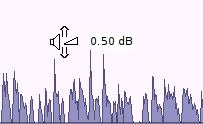
\includegraphics[width=0.4\textwidth]{images/gain-cursor.png}
 \caption{The cursor changes to a gain symbol during the \hact{G} action.}
 \label{fig_gaincursor}
\end{figure}

Up to now we used some simple and easily memorable actions, but there are of course a lot more. But how to know which functions are available for a track or audio clip? Fortunately, there are menus available. You can either use the righ mouse button to popup the menu for the object beneath the mouse cursor, or use \sact{Q} (by now you know that this means pressing the Q key). The menu shows the available functions, and how to perform them on the keyboard (\FigB\ \ref{fig_clipmenu})!

\begin{figure}
 \centering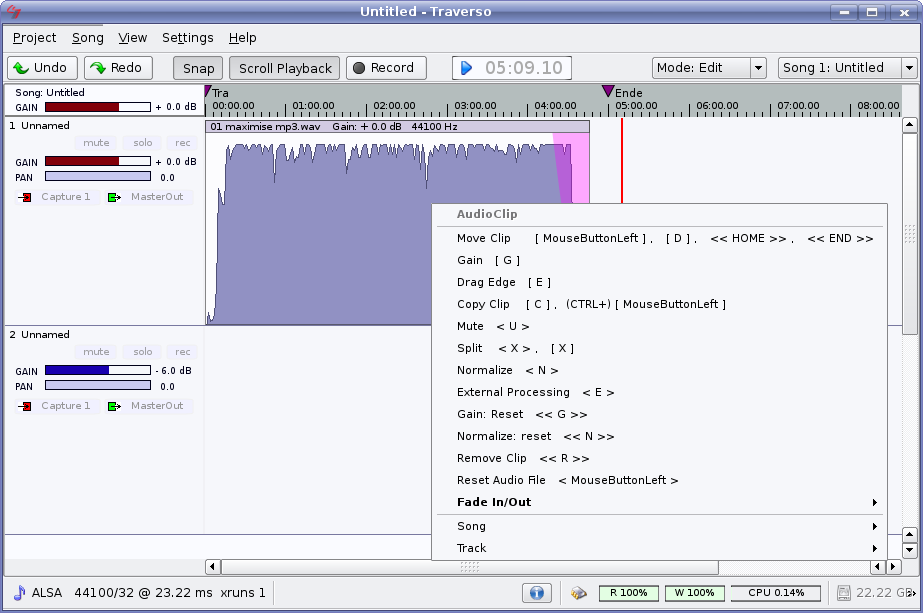
\includegraphics[width=\textwidth]{images/clipmenu.png}
 \caption{Pressing \sact{Q} or the right mouse button on an audio clip shows a menu with all available actions.}
 \label{fig_clipmenu}
\end{figure}

Moving the audio clip can be done by pressing the left mouse button, and keeping it pressed, or by doing the same with the D key. According to our notation scheme that would be \hact{D} or \hact{Left MouseButton}. Alternatively, you can just drag the audio clip with the mousecursor. You can move the mouse freely to position the audio clip to your own liking, the view will automatically scroll if the mouse comes close to the boundaries of the view. Also check out the \hact{Z} and \hact{S} actions to zoom and move the horizontal slider.

By now we learned two kinds of actions, the single key actions \sact{K}, and the hold actions \hact{K}. We also learned that key actions always work on the object beneath the mouse cursor. But before you start exploring the possibilities of Traverso on your own, let's look at some more (randomly selected) functions.

If you want to reset the gain of an audio clip or track to 0 dB, point the mouse cursor to a clip and press the G key twice. This works just like double-clicking with the mouse. In our notation scheme, a double key stroke is notated as \dact{G}. You will see that this action first resets the gain to 0 dB, and if called again, toggles the gain between $-6$ and 0 dB. This also works on the track gain.

As a last example let's delete an audio clip. First select the clip by hitting \sact{S} on it. Its background will become dark. Then hit X and C twice at the same time. This action is difficult to perform, maybe you need a couple of attempts to get it right. But this makes the action ideal for ``dangerous'' function which should by no means happen accidentally. According to our notation scheme this function writes as \dact{X C}. An overview of all available action types is given in chapter \ref{sect_keyactions}. Chapters \ref{sect_recording} and \ref{sect_mixing} provide more detailed information on recording and mixing.

